\section{Day 19: Homotopies (Nov. 12, 2024)}
Outfit of the day: scary uwu
\begin{figure}[h]
    \centering
    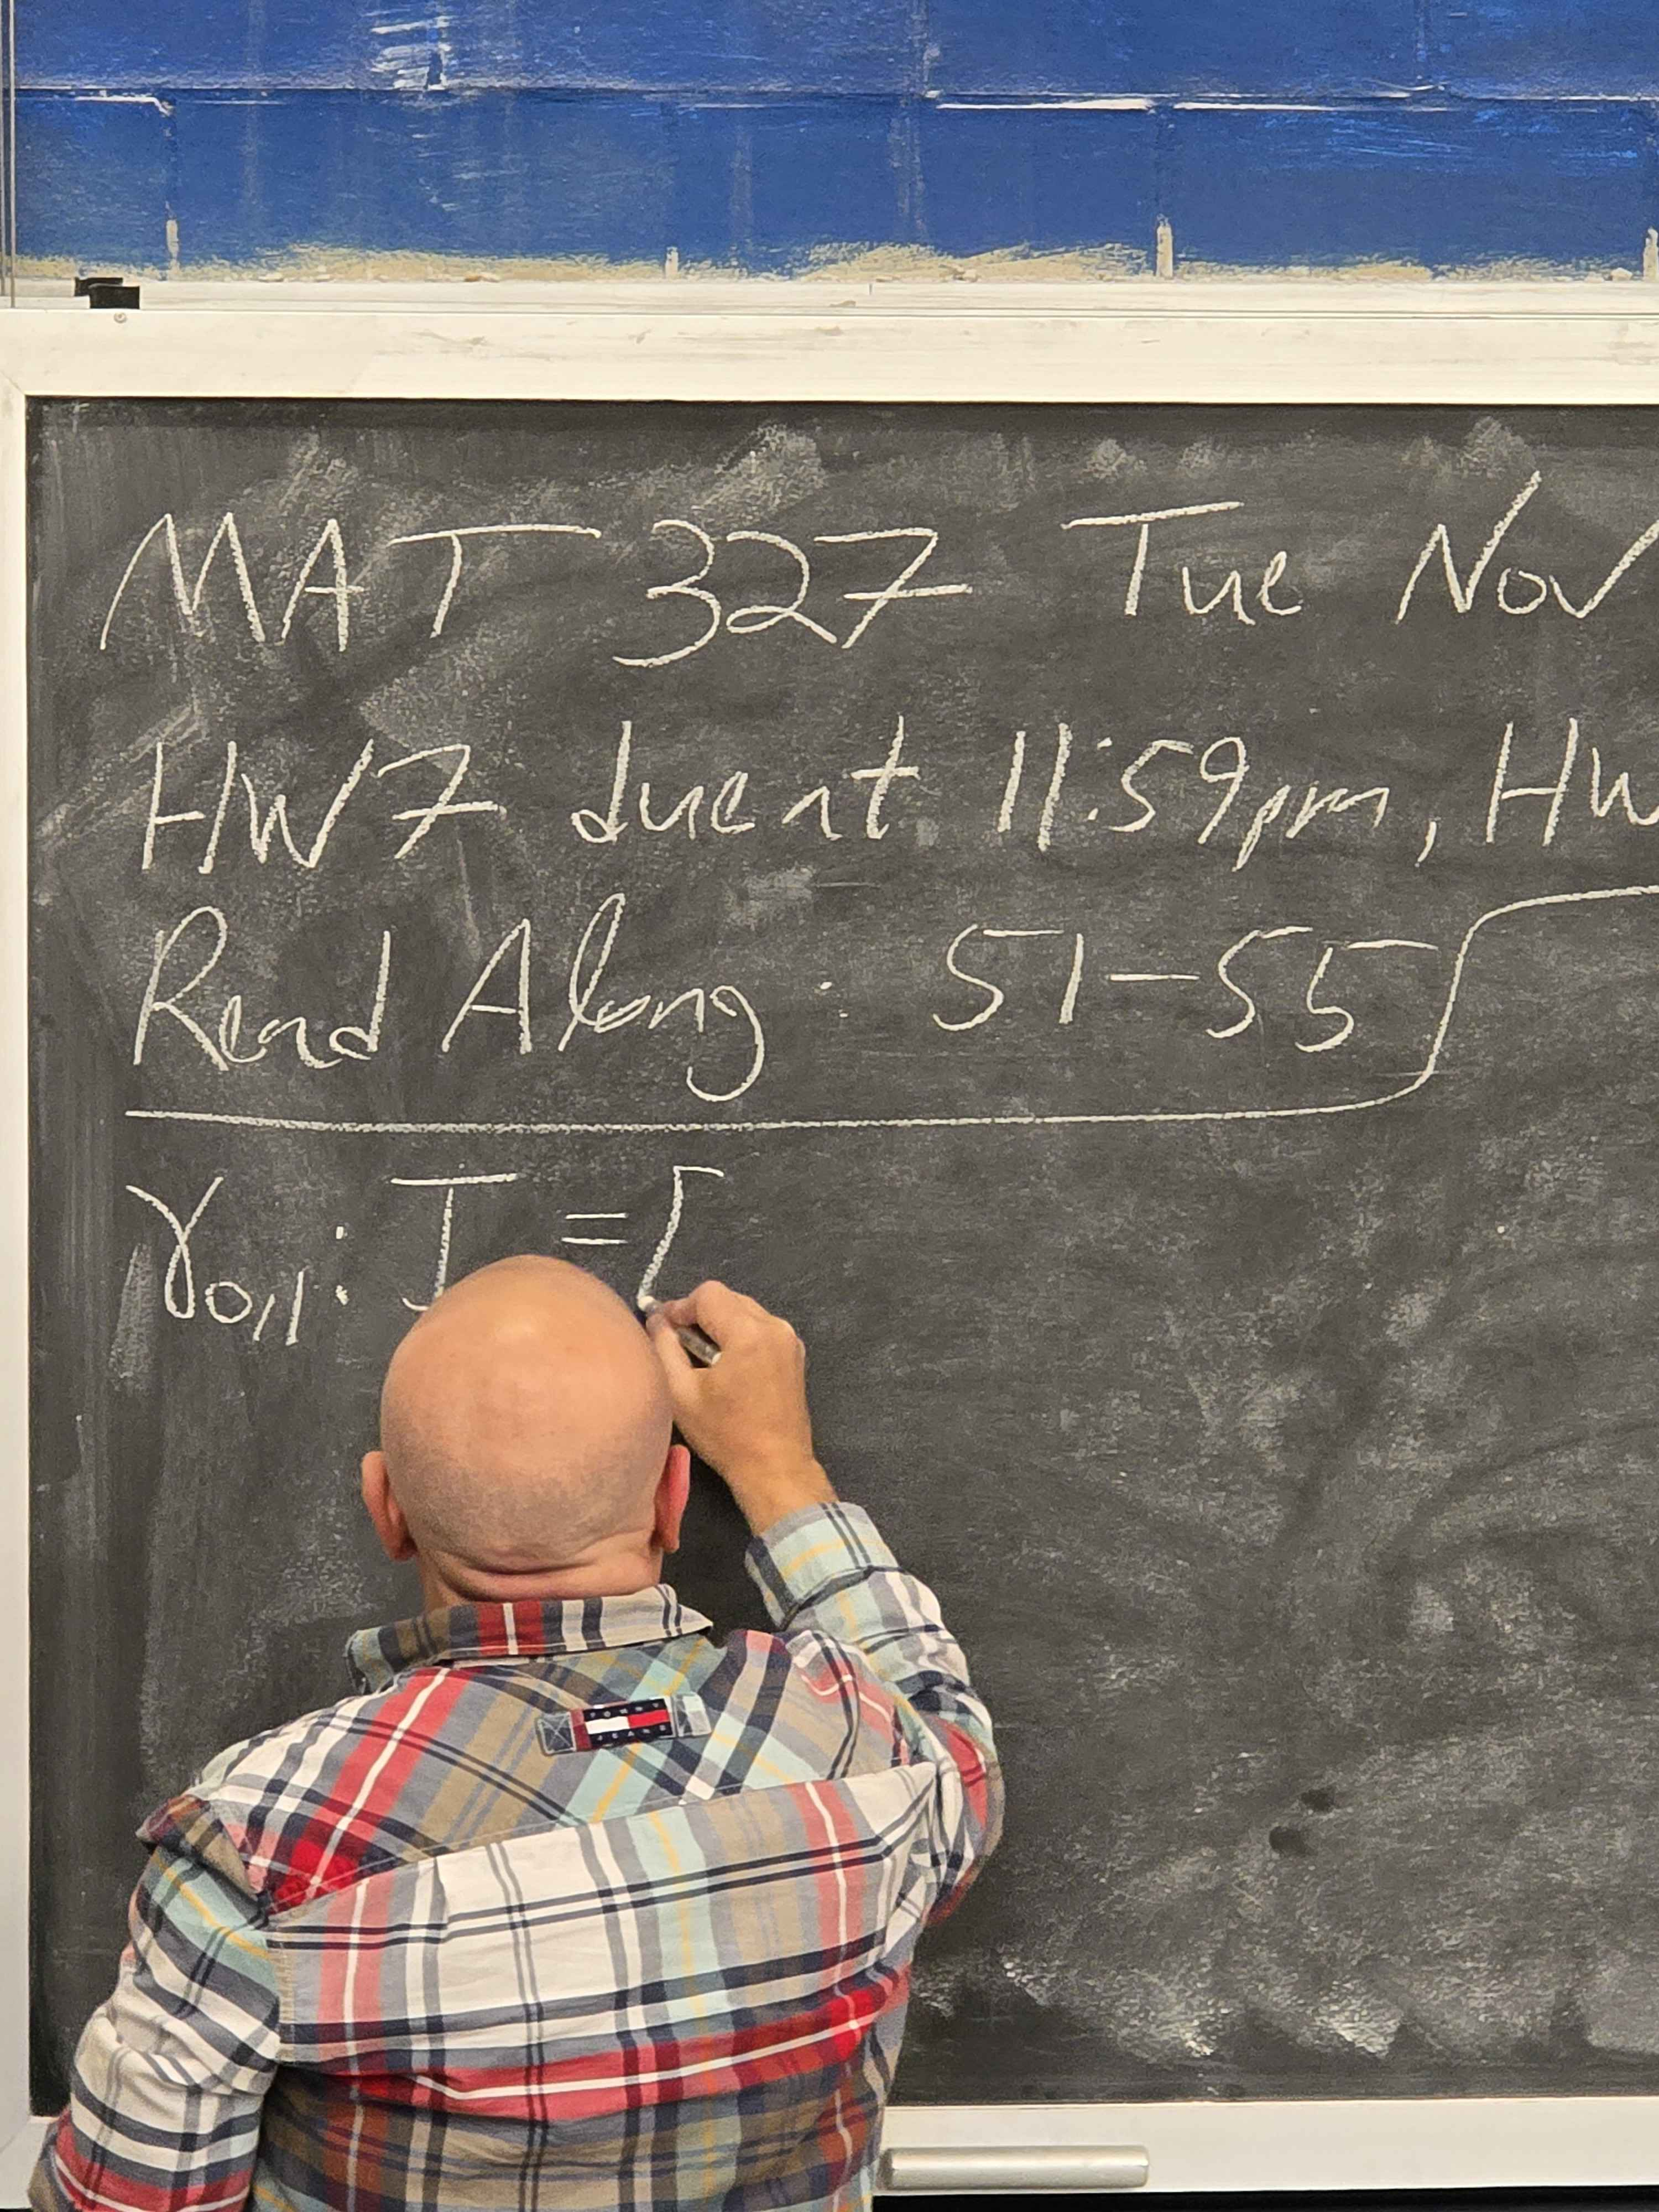
\includegraphics[scale=0.1]{MAT327 Notes/Dror Shirts/dror day 19 shirt.jpg}
\end{figure}

\noindent Recall from last lecture that $\gamma_{0, 1} : I_s \to [0, 1]_s \to X$ and $\gamma_0 \sim_p \gamma_1$ means that path homotopy is an equivalence relation; i.e., there exists $H : I^2_{s, t} \to X$ such that
\begin{align*}
    H(0, t) &= \gamma_0(0) = \gamma_1(0), \\
    H(1, t) &= \gamma_0(1) = \gamma_1(1), \\
    H(s, 0) &= \gamma_0(s), \\
    H(s, 1) &= \gamma_1(s).
\end{align*}
\noindent Let $\gamma : I \to X$ be a path $[\gamma] = \{ \gamma' \mid \gamma' \sim \gamma \}$. $[\gamma]$ is called a homotopy class of paths.
\begin{definition}[Path Composition / Product]
    If $\gamma_1, \gamma_2$ are paths and $\gamma_1(1) = \gamma_2(0)$, then $(\gamma_1 \ast \gamma_2)(s) = \gamma_1(2s)$ when $s \leq \frac{1}{2}$, and $\gamma_2(2s - 1)$ when $s \geq \frac{1}{2}$.
\end{definition}

\newpage
\begin{simpleclaim}
    Path composition descends to homotopy classes of paths; i.e.,
    % https://q.uiver.app/#q=WzAsOCxbMCwwLCJcXHtcXHRleHR7cGF0aHN9XFx9Il0sWzIsMCwiXFx7XFx0ZXh0e3BhdGhzfVxcfSJdLFswLDIsIlxce1xcdGV4dHtob20uIGNsYXNzIG9mIHBhdGhzfVxcfSJdLFsyLDIsIlxce1xcdGV4dHtoLmMuby5wLn1cXH0iXSxbMSwwLCJcXHRpbWVzIl0sWzEsMiwiXFx0aW1lcyJdLFs0LDAsIlxce1xcdGV4dHtwYXRoc31cXH0iXSxbNCwyLCJcXHtcXHRleHR7aC5jLm8ucC59XFx9Il0sWzAsMl0sWzEsM10sWzEsNiwiXFxhc3QiXSxbMyw3LCJcXGFzdCJdLFs2LDddXQ==
    \[\begin{tikzcd}[ampersand replacement=\&,cramped]
        {\{\text{paths}\}} \& \times \& {\{\text{paths}\}} \&\& {\{\text{paths}\}} \\
        \\
        {\{\text{h.c.o.p.}\}} \& \times \& {\{\text{h.c.o.p.}\}} \&\& {\{\text{h.c.o.p.}\}}
        \arrow[from=1-1, to=3-1]
        \arrow["\ast", from=1-3, to=1-5]
        \arrow[from=1-3, to=3-3]
        \arrow[from=1-5, to=3-5]
        \arrow["\ast", from=3-3, to=3-5]
    \end{tikzcd}\]
    where we note that ``h.c.o.p.'' is shorthand for homotopy class of paths. Namely, $[\gamma_1] \ast [\gamma_2] = [\gamma_1 \ast \gamma_2]$ is well-defined. If $\gamma_1 \sim_p \gamma_1'$ and $\gamma_2 \sim_p \gamma_2'$, then we claim that
\[ \gamma_1 \ast \gamma_2 \sim_p \gamma_1' \ast \gamma_2'. \]
\end{simpleclaim}
\noindent We now prove the claim. Assume $\gamma_1 \sim_p^{H_1} \gamma_1'$ and $\gamma_2 \sim_p^{H_1} \gamma_2'$ (read: they are equivalent by the functions $H_1, H_2$ respectively). Then $\gamma_1 \ast \gamma_2 \sim_p^H \gamma_1' \ast \gamma_2'$. If $H_1, H_2$ are the path homotopies of $[\gamma_1], [\gamma_2]$, we may define
\[ H(s, t) = \begin{cases} H_1(2s, t) & s \leq \frac{1}{2}, \\ H_2(2s - 1, t) & s \geq \frac{1}{2}, \end{cases} \]
since $H_1(1, t) = x_1 = H_2(0, t)$ for all $t$. This means $H$ is well-defined, and is continuous by the pasting lemma (Sec. 51, Page 326 in Munkres).
\begin{simplethm}[Theorem 51.2 in Munkres; Groupoid Structure]
    The $\ast$ operation forms a groupoid on the homotopy class of paths, i.e.
    \begin{enumerate}[label=(\alph*)]
        \item $[\gamma_1] \ast ([\gamma_2] \ast [\gamma_3]) = ([\gamma_1] \ast [\gamma_2]) \ast [\gamma_3]$ (associativity),
        \item $[\gamma] \ast [e] = [\gamma] = [e] \ast [\gamma]$ (identity),
        \item there exists $\overline{\gamma}$ for all $\gamma$ such that $[\gamma] \ast [\overline{\gamma}] = [e]$.
    \end{enumerate}
\end{simplethm}
\noindent We check that all the properties hold.
\begin{enumerate}[label=(\alph*)]
    \item For associativity, we have
    \[ [\gamma_1] \ast ([\gamma_2] \ast [\gamma_3]) = [\gamma_1 \ast (\gamma_2 \ast \gamma_3)]; \hspace{0.2in} ([\gamma_1] \ast [\gamma_2]) \ast [\gamma_3] = [(\gamma_1 \ast \gamma_2) \ast \gamma_3]. \]
    Note that $[\gamma_1 \ast (\gamma_2 \ast \gamma_3) \neq (\gamma_1 \ast \gamma_2) \ast \gamma_3$ in general, though, since $\ast$ divides the time parameter in half for each of its inputs, i.e. on the left hand side, we are ``running on'' $\gamma_1$ for half the time and $\gamma_2, \gamma_3$ for a quarter of the time, versus $\gamma_1, \gamma_2$ for a quarter and $\gamma_3$ for half on the RHS.
    \medskip\newline
    There was some diagram that was drawn that concluded the proof. Weird... i'll check textbook later.
    \item Given $x \in X$, let us have $e_x(s) = x$; if $\gamma(0) = x$ and $\gamma(1) = y$, then $[e_x \ast \gamma] = [\gamma \ast e_y] = [\gamma]$.
    \item We now check for inverses. Let $\overline{\gamma}(s) := \gamma(1-s)$. We claim that $[\gamma \ast \overline{\gamma}] = e_x$. More diagram proof. Check Munkres i guess.
\end{enumerate}
